\hypertarget{html-ux7b80ux4ecb}{%
\subsection{HTML 简介}\label{html-ux7b80ux4ecb}}

网页就是
HTML?这么理解大概没错。因为网页中不但包含文字,还有图片、视频、Flash
小游戏,有复杂的排版、动画效果,所以,HTML
定义了一套语法规则,来告诉浏览器如何把一个丰富多彩的页面显示出来。

HTML 长什么样?上次我们看了新浪首页的 HTML 源码,如果仔细数数,竟然有
6000 多行!

所以,学 HTML,就不要指望从新浪入手了。我们来看看最简单的 HTML
长什么样:

\begin{pythoncode}
<html>
<head>
  <title>Hello</title>
</head>
<body>
  <h1>Hello, world!</h1>
</body>
</html>
\end{pythoncode}

可以用文本编辑器编写
HTML,然后保存为\texttt{hello.html},双击或者把文件拖到浏览器中,就可以看到效果:

 
 \begin{figure}[htp]
	\centering
	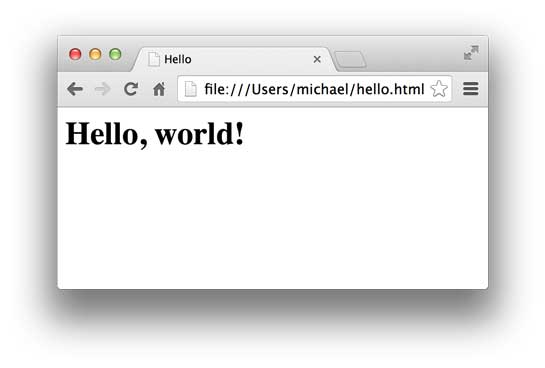
\includegraphics[width=0.6\linewidth]{fig/950569639986880.png}
\end{figure}


HTML 文档就是一系列的 Tag 组成,最外层的 Tag
是\texttt{\textless{}html\textgreater{}}。规范的 HTML
也包含\texttt{\textless{}head\textgreater{}...\textless{}/head\textgreater{}}和\texttt{\textless{}body\textgreater{}...\textless{}/body\textgreater{}}(注意不要和
HTTP 的 Header、Body 搞混了),由于 HTML
是富文档模型,所以,还有一系列的 Tag
用来表示链接、图片、表格、表单等等。

\hypertarget{css-ux7b80ux4ecb}{%
\subsubsection{CSS 简介}\label{css-ux7b80ux4ecb}}

CSS 是 Cascading Style Sheets(层叠样式表)的简称,CSS 用来控制 HTML
里的所有元素如何展现,比如,给标题元素\texttt{\textless{}h1\textgreater{}}加一个样式,变成
48 号字体,灰色,带阴影:

\begin{pythoncode}
<html>
<head>
  <title>Hello</title>
  <style>
    h1 {
      color: #333333;
      font-size: 48px;
      text-shadow: 3px 3px 3px #666666;
    }
  </style>
</head>
<body>
  <h1>Hello, world!</h1>
</body>
</html>
\end{pythoncode}

效果如下:

 
 \begin{figure}[htp]
	\centering
	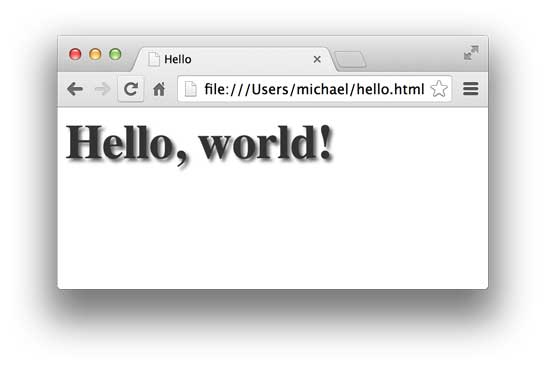
\includegraphics[width=0.6\linewidth]{fig/950571217609344.png}
\end{figure}


\hypertarget{javascript-ux7b80ux4ecb}{%
\subsubsection{JavaScript 简介}\label{javascript-ux7b80ux4ecb}}

JavaScript 虽然名称有个 Java,但它和 Java 真的一点关系没有。JavaScript
是为了让 HTML 具有交互性而作为脚本语言添加的,JavaScript 既可以内嵌到
HTML 中,也可以从外部链接到 HTML
中。如果我们希望当用户点击标题时把标题变成红色,就必须通过 JavaScript
来实现:

\begin{pythoncode}
<html>
<head>
  <title>Hello</title>
  <style>
    h1 {
      color: #333333;
      font-size: 48px;
      text-shadow: 3px 3px 3px #666666;
    }
  </style>
  <script>
    function change() {
      document.getElementsByTagName('h1')[0].style.color = '#ff0000';
    }
  </script>
</head>
<body>
  <h1 onclick="change()">Hello, world!</h1>
</body>
</html>
\end{pythoncode}

点击标题后效果如下:

 
 \begin{figure}[htp]
	\centering
	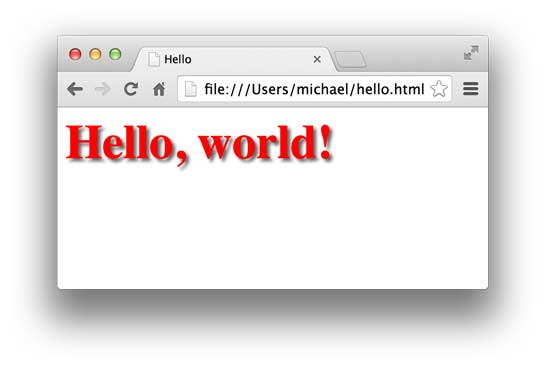
\includegraphics[width=0.6\linewidth]{fig/950572257640320.png}
\end{figure}


\hypertarget{ux5c0fux7ed3}{%
\subsubsection{小结}\label{ux5c0fux7ed3}}

如果要学习 Web 开发,首先要对 HTML、CSS 和 JavaScript 作一定的了解。HTML
定义了页面的内容,CSS 来控制页面元素的样式,而 JavaScript
负责页面的交互逻辑。

讲解 HTML、CSS 和 JavaScript 就可以写 3 本书,对于优秀的 Web
开发人员来说,精通 HTML、CSS 和 JavaScript
是必须的,这里推荐一个在线学习网站 w3schools:

\url{http://www.w3schools.com/}

以及一个对应的中文版本:

\url{http://www.w3school.com.cn/}

当我们用 Python 或者其他语言开发 Web
应用时,我们就是要在服务器端动态创建出
HTML,这样,浏览器就会向不同的用户显示出不同的 Web 页面。

